\usetikzlibrary{patterns}
\begin{figure*}[t!]
  \centering
  % 第一行:两图并排
  \ref{sharedlegend}
  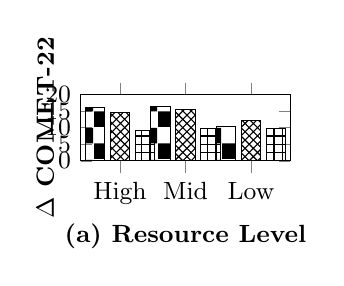
\begin{tikzpicture}
    \begin{axis}[
      ybar,
      bar width=7pt,  % 让 bar 变宽以填充空隙
      width=0.35\textwidth,
      height=0.20\textwidth,
      xlabel={\small{(a) Resource Level}},
      ylabel={\small{$\Delta$ COMET-22}},
      xlabel style={font=\bfseries},
      ylabel style={font=\bfseries,yshift=-1em},
      symbolic x coords={High, Mid, Low},
      xtick=data,
      xticklabel style={font=\small},
      yticklabel style={font=\small},
      ymin=0, ymax=20,
      % nodes near coords,
      % nodes near coords style={font=\tiny},
      enlarge x limits=0.3,  % 确保不同类别间有间距
      legend style={
        draw=none,
        fill=none,
        font=\small,
        column sep=0.3cm,
        at={(1,3.7)},
        anchor=north
      },
      legend columns=3,
      legend to name=sharedlegend
    ]
      \addplot[fill=red!80, pattern=checkerboard] coordinates {(High, 16.106) (Mid, 16.28) (Low, 10.279)};
      \addlegendentry{ALMA-7B-Pretrain}
      \addplot[fill=blue!80, pattern=crosshatch] coordinates {(High, 14.548) (Mid, 15.438) (Low, 12.061)};
      \addlegendentry{ALMA-13B-Pretrain}
      \addplot[fill=green!80, pattern=grid] coordinates {(High, 9.1) (Mid, 9.8) (Low, 9.657)};
      \addlegendentry{X-ALMA-13B-Pretrain}
    \end{axis}
  \end{tikzpicture}
  \hspace{0.3cm}
  % 第二行:单图居中
  \vspace{0.2cm}
  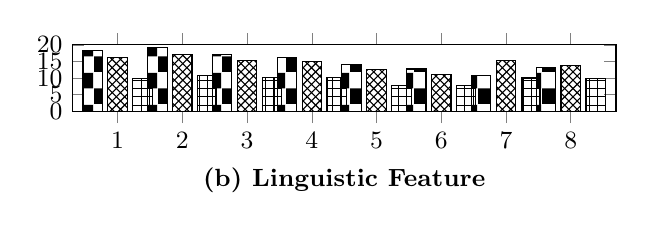
\begin{tikzpicture}
    \begin{axis}[
      ybar,
      bar width=7pt,  
      width=0.7\textwidth,
      height=0.20\textwidth,
      xlabel={\small{(b) Linguistic Feature}},
      xlabel style={font=\bfseries},
      symbolic x coords={1, 2, 3, 4, 5, 6, 7, 8},
      xtick=data,
      xticklabel style={font=\small},
      yticklabel style={font=\small},
      ymin=0, ymax=20,
      % nodes near coords,
      % nodes near coords style={font=\tiny},
      enlarge x limits=0.1,  
    ]
      \addplot[fill=red!80, pattern=checkerboard] coordinates {
        (1, 18.34) (2, 19.202) (3, 17.138) 
        (4, 16.182) (5, 14.224) 
        (6, 12.734) (7, 10.686) (8, 13.285)};
      \addplot[fill=blue!80, pattern=crosshatch] coordinates {
        (1, 16.12) (2, 17.19) (3, 15.22) 
        (4, 14.88) (5, 12.56) 
        (6, 11.2) (7, 15.33) (8, 13.73)};
      \addplot[fill=green!80, pattern=grid] coordinates {
        (1, 9.99) (2, 10.66) (3, 10.23) 
        (4, 10.12) (5, 7.66) 
        (6, 7.73) (7, 10.03) (8, 10.02)};
    \end{axis}
  \end{tikzpicture}
  \vskip -0.2in
  \caption{$\Delta$ COMET-22 between separate training and multilingual training in XX → En translation, grouped by resource level and linguistic features. The magnitude of $\Delta$ COMET-22 denotes the intensity of linguistic conflicts.}
  \label{fig:performance_gap_vs_language_group_and_resource_level}
\end{figure*}
